
\documentclass[convert={outext=.jpg}]{standalone}
\usepackage{ulem,tikz,amsmath}
\usetikzlibrary{positioning}

\begin{document}
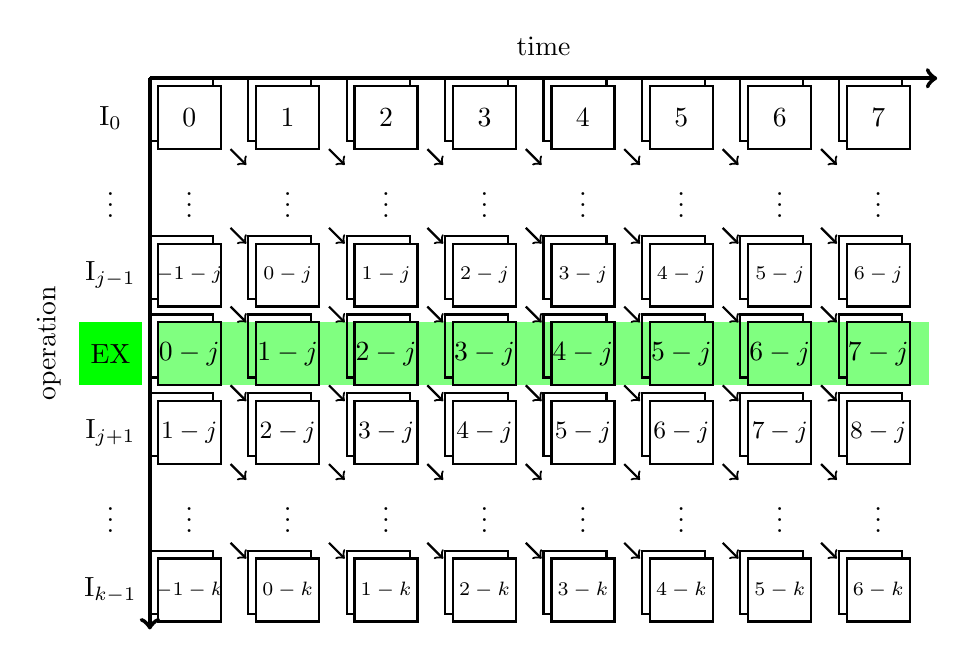
\begin{tikzpicture}[thick]
  \draw [ultra thick,->] (0, 1) -- (10, 1) node[midway, label={time}] {};
  \path (-1, 1) -- (-1,-6) node[midway, label={[rotate=90]operation}] {};
  \draw [ultra thick,->] (0, 1) -- (0,-6);
  \fill[green] (-0.9,-2.1) rectangle ++(0.8,-0.8);
  \fill[green!50!white] (0.1,-2.1) rectangle ++(9.8,-0.8); \path (-0.5,0.5) node {$\text{I}_{0}$}
      ++(0,-1) node {$\vdots$}
      ++(0,-1) node {$\text{I}_{j-1}$}
      ++(0,-1) node {EX}
      ++(0,-1) node {$\text{I}_{j+1}$}
      ++(0,-1) node {$\vdots$}
      ++(0,-1) node {$\text{I}_{k-1}$};

  \foreach \x in {0,...,7}
    {%
      \draw (1.25*\x, 1) +(0.1,-0.8) -- +(0.0,-0.8) -- +(0.0, 0.0) -- +(0.8,-0.0) -- +(0.8,-0.1) +(0.1,-0.1) rectangle +(0.9,-0.9) node[midway]{\x};
      \draw (1.25*\x, 0) +(0.5,-0.5) node {$\vdots$};
      \pgfmathsetmacro\atext{\x - 1}
      \draw (1.25*\x, -1) +(0.1,-0.8) -- +(0.0,-0.8) -- +(0.0, 0.0) -- +(0.8,-0.0) -- +(0.8,-0.1) +(0.1,-0.1) rectangle +(0.9,-0.9) node[midway]{\scriptsize$\pgfmathprintnumber{\atext} - j$};
      \draw (1.25*\x, -2) +(0.1,-0.8) -- +(0.0,-0.8) -- +(0.0, 0.0) -- +(0.8,-0.0) -- +(0.8,-0.1) +(0.1,-0.1) rectangle +(0.9,-0.9) node[midway]{$\x - j$};
      \pgfmathsetmacro\atext{\x + 1}
      \draw (1.25*\x, -3) +(0.1,-0.8) -- +(0.0,-0.8) -- +(0.0, 0.0) -- +(0.8,-0.0) -- +(0.8,-0.1) +(0.1,-0.1) rectangle +(0.9,-0.9) node[midway]{\small$\pgfmathprintnumber{\atext} - j$};
      \draw (1.25*\x, -4) +(0.5,-0.5) node {$\vdots$};
      \pgfmathsetmacro\atext{\x - 1}
      \draw (1.25*\x, -5) +(0.1,-0.8) -- +(0.0,-0.8) -- +(0.0, 0.0) -- +(0.8,-0.0) -- +(0.8,-0.1) +(0.1,-0.1) rectangle +(0.9,-0.9) node[midway]{\scriptsize$\pgfmathprintnumber{\atext} - k$};
    }%;
  \foreach \x in {0,...,6}
    \foreach \y in {0,...,5}
      \draw [->] (1.25*\x,1-\y) +(1.025,-0.9) -- +(1.225,-1.1);
\end{tikzpicture}
\end{document}
